\documentclass{standalone}
\usepackage{tikz}
\usetikzlibrary{patterns, positioning}


\begin{document}
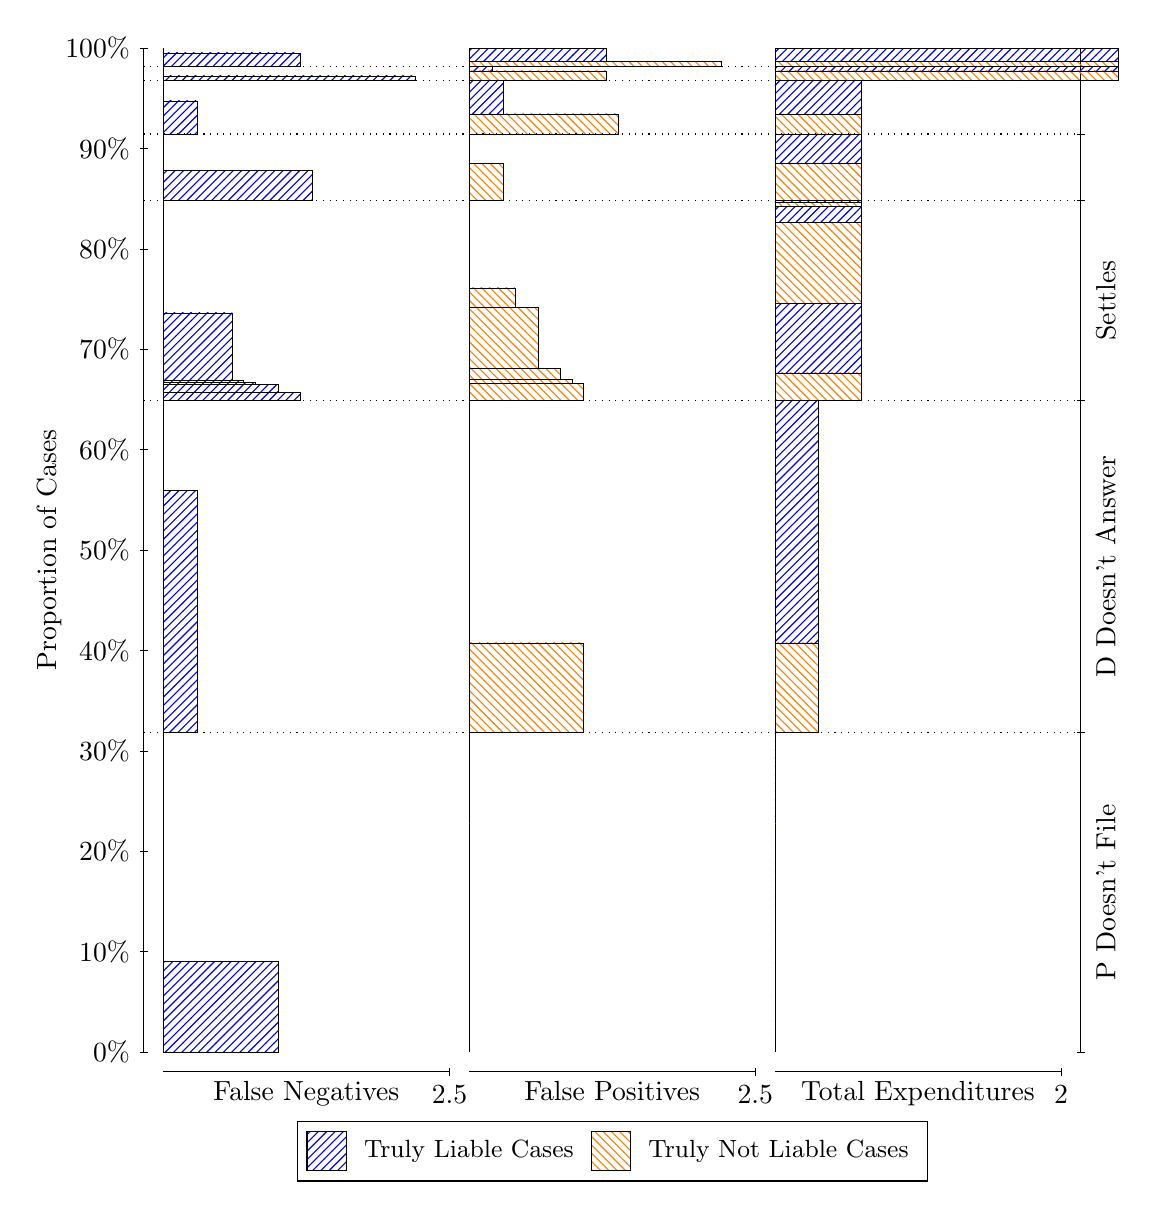
\begin{tikzpicture}
\draw[black, very thin] (1.5,1.75) -- (1.5,14.5);
\node[rotate=90, text=black, anchor=center] at (0.3, 8.125) {Proportion of Cases};
\draw[black, very thin] (1.45,1.75) -- (1.55,1.75);
\node[text=black, anchor=east] at (1.45, 1.75) {0\%};
\draw[black, very thin] (1.45,3.025) -- (1.55,3.025);
\node[text=black, anchor=east] at (1.45, 3.025) {10\%};
\draw[black, very thin] (1.45,4.3) -- (1.55,4.3);
\node[text=black, anchor=east] at (1.45, 4.3) {20\%};
\draw[black, very thin] (1.45,5.575) -- (1.55,5.575);
\node[text=black, anchor=east] at (1.45, 5.575) {30\%};
\draw[black, very thin] (1.45,6.85) -- (1.55,6.85);
\node[text=black, anchor=east] at (1.45, 6.85) {40\%};
\draw[black, very thin] (1.45,8.125) -- (1.55,8.125);
\node[text=black, anchor=east] at (1.45, 8.125) {50\%};
\draw[black, very thin] (1.45,9.4) -- (1.55,9.4);
\node[text=black, anchor=east] at (1.45, 9.4) {60\%};
\draw[black, very thin] (1.45,10.675) -- (1.55,10.675);
\node[text=black, anchor=east] at (1.45, 10.675) {70\%};
\draw[black, very thin] (1.45,11.95) -- (1.55,11.95);
\node[text=black, anchor=east] at (1.45, 11.95) {80\%};
\draw[black, very thin] (1.45,13.225) -- (1.55,13.225);
\node[text=black, anchor=east] at (1.45, 13.225) {90\%};
\draw[black, very thin] (1.45,14.5) -- (1.55,14.5);
\node[text=black, anchor=east] at (1.45, 14.5) {100\%};

\draw[black, very thin] (13.4,1.75) -- (13.4,14.5);
\draw[black, very thin] (13.35,1.75) -- (13.45,1.75);
\node[anchor=west] at (13.35, 1.75) {};
\draw[black, very thin] (13.35,5.8056) -- (13.45,5.8056);
\node[anchor=west] at (13.35, 5.8056) {};
\draw[black, very thin] (13.35,10.024) -- (13.45,10.024);
\node[anchor=west] at (13.35, 10.024) {};
\draw[black, very thin] (13.35,12.567) -- (13.45,12.567);
\node[anchor=west] at (13.35, 12.567) {};
\draw[black, very thin] (13.35,13.408) -- (13.45,13.408);
\node[anchor=west] at (13.35, 13.408) {};
\draw[black, very thin] (13.35,14.085) -- (13.45,14.085);
\node[anchor=west] at (13.35, 14.085) {};
\draw[black, very thin] (13.35,14.27) -- (13.45,14.27);
\node[anchor=west] at (13.35, 14.27) {};
\draw[black, very thin] (13.35,14.5) -- (13.45,14.5);
\node[anchor=west] at (13.35, 14.5) {};

\draw[black, very thin, pattern color=blue, pattern=north east lines] (1.75,1.75) rectangle (3.2033,2.9052);
\draw[black, very thin, pattern color=orange, pattern=north west lines] (1.75,2.9052) rectangle (1.75,5.8056);
\draw[black, very thin, pattern color=blue, pattern=north east lines] (1.75,5.8056) rectangle (2.186,8.8843);
\draw[black, very thin, pattern color=orange, pattern=north west lines] (1.75,8.8843) rectangle (1.75,10.024);
\draw[black, very thin, pattern color=blue, pattern=north east lines] (1.75,10.024) rectangle (3.494,10.129);
\draw[black, very thin, pattern color=blue, pattern=north east lines] (1.75,10.129) rectangle (3.2033,10.226);
\draw[black, very thin, pattern color=blue, pattern=north east lines] (1.75,10.226) rectangle (2.9127,10.252);
\draw[black, very thin, pattern color=blue, pattern=north east lines] (1.75,10.252) rectangle (2.7673,10.281);
\draw[black, very thin, pattern color=blue, pattern=north east lines] (1.75,10.281) rectangle (2.622,11.137);
\draw[black, very thin, pattern color=orange, pattern=north west lines] (1.75,11.137) rectangle (1.75,12.567);
\draw[black, very thin, pattern color=blue, pattern=north east lines] (1.75,12.567) rectangle (3.6393,12.944);
\draw[black, very thin, pattern color=orange, pattern=north west lines] (1.75,12.944) rectangle (1.75,13.408);
\draw[black, very thin, pattern color=blue, pattern=north east lines] (1.75,13.408) rectangle (2.186,13.829);
\draw[black, very thin, pattern color=orange, pattern=north west lines] (1.75,13.829) rectangle (1.75,14.085);
\draw[black, very thin, pattern color=blue, pattern=north east lines] (1.75,14.085) rectangle (4.9473,14.146);
\draw[black, very thin, pattern color=orange, pattern=north west lines] (1.75,14.146) rectangle (1.75,14.27);
\draw[black, very thin, pattern color=blue, pattern=north east lines] (1.75,14.27) rectangle (3.494,14.439);
\draw[black, very thin, pattern color=orange, pattern=north west lines] (1.75,14.439) rectangle (1.75,14.5);
\draw[black, very thin, pattern color=orange, pattern=north west lines] (5.6333,1.75) rectangle (5.6333,4.6504);
\draw[black, very thin, pattern color=blue, pattern=north east lines] (5.6333,4.6504) rectangle (5.6333,5.8056);
\draw[black, very thin, pattern color=orange, pattern=north west lines] (5.6333,5.8056) rectangle (7.0867,6.9453);
\draw[black, very thin, pattern color=blue, pattern=north east lines] (5.6333,6.9453) rectangle (5.6333,10.024);
\draw[black, very thin, pattern color=orange, pattern=north west lines] (5.6333,10.024) rectangle (7.0867,10.24);
\draw[black, very thin, pattern color=orange, pattern=north west lines] (5.6333,10.24) rectangle (6.9413,10.292);
\draw[black, very thin, pattern color=orange, pattern=north west lines] (5.6333,10.292) rectangle (6.796,10.427);
\draw[black, very thin, pattern color=orange, pattern=north west lines] (5.6333,10.427) rectangle (6.5053,11.202);
\draw[black, very thin, pattern color=orange, pattern=north west lines] (5.6333,11.202) rectangle (6.2147,11.454);
\draw[black, very thin, pattern color=blue, pattern=north east lines] (5.6333,11.454) rectangle (5.6333,12.567);
\draw[black, very thin, pattern color=orange, pattern=north west lines] (5.6333,12.567) rectangle (6.0693,13.031);
\draw[black, very thin, pattern color=blue, pattern=north east lines] (5.6333,13.031) rectangle (5.6333,13.408);
\draw[black, very thin, pattern color=orange, pattern=north west lines] (5.6333,13.408) rectangle (7.5227,13.664);
\draw[black, very thin, pattern color=blue, pattern=north east lines] (5.6333,13.664) rectangle (6.0693,14.085);
\draw[black, very thin, pattern color=orange, pattern=north west lines] (5.6333,14.085) rectangle (7.3773,14.209);
\draw[black, very thin, pattern color=blue, pattern=north east lines] (5.6333,14.209) rectangle (5.924,14.27);
\draw[black, very thin, pattern color=orange, pattern=north west lines] (5.6333,14.27) rectangle (8.8307,14.331);
\draw[black, very thin, pattern color=blue, pattern=north east lines] (5.6333,14.331) rectangle (7.3773,14.5);
\draw[black, very thin, pattern color=orange, pattern=north west lines] (9.5167,1.75) rectangle (9.5167,4.6504);
\draw[black, very thin, pattern color=blue, pattern=north east lines] (9.5167,4.6504) rectangle (9.5167,5.8056);
\draw[black, very thin, pattern color=orange, pattern=north west lines] (9.5167,5.8056) rectangle (10.062,6.9453);
\draw[black, very thin, pattern color=blue, pattern=north east lines] (9.5167,6.9453) rectangle (10.062,10.024);
\draw[black, very thin, pattern color=orange, pattern=north west lines] (9.5167,10.024) rectangle (10.607,10.375);
\draw[black, very thin, pattern color=blue, pattern=north east lines] (9.5167,10.375) rectangle (10.607,11.256);
\draw[black, very thin, pattern color=orange, pattern=north west lines] (9.5167,11.256) rectangle (10.607,12.283);
\draw[black, very thin, pattern color=blue, pattern=north east lines] (9.5167,12.283) rectangle (10.607,12.485);
\draw[black, very thin, pattern color=orange, pattern=north west lines] (9.5167,12.485) rectangle (10.607,12.538);
\draw[black, very thin, pattern color=blue, pattern=north east lines] (9.5167,12.538) rectangle (10.607,12.567);
\draw[black, very thin, pattern color=orange, pattern=north west lines] (9.5167,12.567) rectangle (10.607,13.031);
\draw[black, very thin, pattern color=blue, pattern=north east lines] (9.5167,13.031) rectangle (10.607,13.408);
\draw[black, very thin, pattern color=orange, pattern=north west lines] (9.5167,13.408) rectangle (10.607,13.664);
\draw[black, very thin, pattern color=blue, pattern=north east lines] (9.5167,13.664) rectangle (10.607,14.085);
\draw[black, very thin, pattern color=orange, pattern=north west lines] (9.5167,14.085) rectangle (13.877,14.209);
\draw[black, very thin, pattern color=blue, pattern=north east lines] (9.5167,14.209) rectangle (13.877,14.27);
\draw[black, very thin, pattern color=orange, pattern=north west lines] (9.5167,14.27) rectangle (13.877,14.331);
\draw[black, very thin, pattern color=blue, pattern=north east lines] (9.5167,14.331) rectangle (13.877,14.5);
\draw[black, dotted] (1.5,5.8056) -- (13.4,5.8056);
\draw[black, dotted] (1.5,10.024) -- (13.4,10.024);
\draw[black, dotted] (1.5,12.567) -- (13.4,12.567);
\draw[black, dotted] (1.5,13.408) -- (13.4,13.408);
\draw[black, dotted] (1.5,14.085) -- (13.4,14.085);
\draw[black, dotted] (1.5,14.27) -- (13.4,14.27);
\draw[black, very thin] (1.75,1.5) -- (5.3833,1.5);
\node[text=black, anchor=north] at (3.5667, 1.5) {False Negatives};
\draw[black, very thin] (5.3833,1.45) -- (5.3833,1.55);
\node[text=black, anchor=north] at (5.3833, 1.45) {2.5};

\draw[black, very thin] (5.6333,1.5) -- (9.2667,1.5);
\node[text=black, anchor=north] at (7.45, 1.5) {False Positives};
\draw[black, very thin] (9.2667,1.45) -- (9.2667,1.55);
\node[text=black, anchor=north] at (9.2667, 1.45) {2.5};

\draw[black, very thin] (9.5167,1.5) -- (13.15,1.5);
\node[text=black, anchor=north] at (11.333, 1.5) {Total Expenditures};
\draw[black, very thin] (13.15,1.45) -- (13.15,1.55);
\node[text=black, anchor=north] at (13.15, 1.45) {2};

\node[text=black, centered, rotate=90] at (13.72, 3.7778) {P Doesn't File};
\node[text=black, centered, rotate=90] at (13.72, 7.9148) {D Doesn't Answer};
\node[text=black, centered, rotate=90] at (13.72, 11.295) {Settles};





\draw (7.449999999999999,1.5) node[draw=none] (baseCoordinate) {};
\begin{scope}[align=center]
        \matrix[scale=0.5, draw=black, below=0.5cm of baseCoordinate, nodes={draw}, column sep=0.1cm]{
            \node[rectangle, draw, minimum width=0.5cm, minimum height=0.5cm, pattern color=blue, pattern=north east lines] {}; &
            \node[draw=none, font=\small, text=black] (B) {Truly Liable Cases}; &
            \node[rectangle, draw, minimum width=0.5cm, minimum height=0.5cm, pattern color=orange, pattern=north west lines] {}; &
            \node[draw=none, font=\small, text=black] (B) {Truly Not Liable Cases}; \\
            };
\end{scope}

\end{tikzpicture}
\end{document}